%%%%%%%%%%%%%%%%%%%%%%%%%%%%%%%%%%%%%%%%%
% Masters/Doctoral Thesis 
% LaTeX Template
% Version 2.5 (27/8/17)
%
% This template was downloaded from:
% http://www.LaTeXTemplates.com
%
% Version 2.x major modifications by:
% Vel (vel@latextemplates.com)
%
% This template is based on a template by:
% Steve Gunn (http://users.ecs.soton.ac.uk/srg/softwaretools/document/templates/)
% Sunil Patel (http://www.sunilpatel.co.uk/thesis-template/)
%
% Template license:
% CC BY-NC-SA 3.0 (http://creativecommons.org/licenses/by-nc-sa/3.0/)
%
%%%%%%%%%%%%%%%%%%%%%%%%%%%%%%%%%%%%%%%%%

%----------------------------------------------------------------------------------------
%  TEMPLATE PACKAGES
%----------------------------------------------------------------------------------------

\documentclass[
11pt, % The default document font size, options: 10pt, 11pt, 12pt
%oneside, % Two side (alternating margins) for binding by default, uncomment to switch to one side
english, % ngerman for German
singlespacing, % Single line spacing, alternatives: onehalfspacing or doublespacing
%draft, % Uncomment to enable draft mode (no pictures, no links, overfull hboxes indicated)
%nolistspacing, % If the document is onehalfspacing or doublespacing, uncomment this to set spacing in lists to single
%liststotoc, % Uncomment to add the list of figures/tables/etc to the table of contents
%toctotoc, % Uncomment to add the main table of contents to the table of contents
%parskip, % Uncomment to add space between paragraphs
%nohyperref, % Uncomment to not load the hyperref package
headsepline, % Uncomment to get a line under the header
%chapterinoneline, % Uncomment to place the chapter title next to the number on one line
%consistentlayout, % Uncomment to change the layout of the declaration, abstract and acknowledgements pages to match the default layout
]{MastersDoctoralThesis} % The class file specifying the document structure

\usepackage[utf8]{inputenc} % Required for inputting international characters
\usepackage[T1]{fontenc} % Output font encoding for international characters
\usepackage{mathpazo} % Use the Palatino font by default
\usepackage[backend=biber,style=authoryear,natbib=true]{biblatex} % or backend=bibtex
\usepackage[autostyle=true]{csquotes} % Required to generate language-dependent quotes in the bibliography
\addbibresource{Bibliography.bib} % The filename of the bibliography

%----------------------------------------------------------------------------------------
%  ADDITIONAL PACKAGES
%----------------------------------------------------------------------------------------

\usepackage{xargs}

\usepackage{xcolor}

\usepackage[colorinlistoftodos,prependcaption,textsize=tiny]{todonotes}

\usepackage{siunitx}
%\sisetup{mode=text,range-phrase = {\text{~to~}}}
\sisetup{
  detect-weight = true,
  range-phrase = {,}\ ,
  range-units  = brackets,
  open-bracket = [,
  close-bracket= ],
}

\usepackage{threeparttable}

%\usepackage{emptypage}

\usepackage{bm}

\usepackage{textcomp}

\usepackage{listings}
\lstset{
  language=Octave,
  morecomment = [l][\itshape\color{blue}]{\#}
}

%----------------------------------------------------------------------------------------
%  NEW COMMANDS
%----------------------------------------------------------------------------------------

\newcommandx{\noteseb}[2][1=]{\todo[linecolor=blue,backgroundcolor=blue!25,bordercolor=blue,#1]{#2}}
\newcommand{\colseb}[1]{{\color{blue} Seb: #1}}

%----------------------------------------------------------------------------------------
%  MARGIN SETTINGS
%----------------------------------------------------------------------------------------

\geometry{
  paper=a4paper, % Change to letterpaper for US letter
  inner=2.5cm, % Inner margin
  outer=3.8cm, % Outer margin
  bindingoffset=.5cm, % Binding offset
  top=1.5cm, % Top margin
  bottom=1.5cm, % Bottom margin
  marginparwidth=100pt,
  %showframe, % Uncomment to show how the type block is set on the page
}

%----------------------------------------------------------------------------------------
%  THESIS INFORMATION
%----------------------------------------------------------------------------------------

\thesistitle{Thesis Title} % Your thesis title, this is used in the title and abstract, print it elsewhere with \ttitle
\supervisor{Dr. James \textsc{Smith}} % Your supervisor's name, this is used in the title page, print it elsewhere with \supname
\examiner{} % Your examiner's name, this is not currently used anywhere in the template, print it elsewhere with \examname
\degree{Doctor of Philosophy} % Your degree name, this is used in the title page and abstract, print it elsewhere with \degreename
\author{John \textsc{Smith}} % Your name, this is used in the title page and abstract, print it elsewhere with \authorname
\addresses{} % Your address, this is not currently used anywhere in the template, print it elsewhere with \addressname

\subject{Biological Sciences} % Your subject area, this is not currently used anywhere in the template, print it elsewhere with \subjectname
\keywords{} % Keywords for your thesis, this is not currently used anywhere in the template, print it elsewhere with \keywordnames
\university{\href{http://www.university.com}{University Name}} % Your university's name and URL, this is used in the title page and abstract, print it elsewhere with \univname
\department{\href{http://department.university.com}{Department or School Name}} % Your department's name and URL, this is used in the title page and abstract, print it elsewhere with \deptname
\group{\href{http://researchgroup.university.com}{Research Group Name}} % Your research group's name and URL, this is used in the title page, print it elsewhere with \groupname
\faculty{\href{http://faculty.university.com}{Faculty Name}} % Your faculty's name and URL, this is used in the title page and abstract, print it elsewhere with \facname

\AtBeginDocument{
\hypersetup{pdftitle=\ttitle} % Set the PDF's title to your title
\hypersetup{pdfauthor=\authorname} % Set the PDF's author to your name
\hypersetup{pdfkeywords=\keywordnames} % Set the PDF's keywords to your keywords
}

\begin{document}

\frontmatter % Use roman page numbering style (i, ii, iii, iv...) for the pre-content pages

\pagestyle{plain} % Default to the plain heading style until the thesis style is called for the body content

%----------------------------------------------------------------------------------------
%  TITLE PAGE
%----------------------------------------------------------------------------------------

\begin{titlepage}
\begin{center}

\vspace*{.06\textheight}
{\scshape\LARGE \univname\par}\vspace{1.5cm} % University name
\textsc{\Large Doctoral Thesis}\\[0.5cm] % Thesis type

\HRule \\[0.4cm] % Horizontal line
{\huge \bfseries \ttitle\par}\vspace{0.4cm} % Thesis title
\HRule \\[1.5cm] % Horizontal line
 
\begin{minipage}[t]{0.4\textwidth}
\begin{flushleft} \large
\emph{Author:}\\
\href{http://www.johnsmith.com}{\authorname} % Author name - remove the \href bracket to remove the link
\end{flushleft}
\end{minipage}
\begin{minipage}[t]{0.4\textwidth}
\begin{flushright} \large
\emph{Supervisor:} \\
\href{http://www.jamessmith.com}{\supname} % Supervisor name - remove the \href bracket to remove the link  
\end{flushright}
\end{minipage}\\[3cm]
 
\vfill

\large \textit{A thesis submitted in fulfillment of the requirements\\ for the degree of \degreename}\\[0.3cm] % University requirement text
\textit{in the}\\[0.4cm]
\groupname\\\deptname\\[2cm] % Research group name and department name
 
\vfill

{\large \today}\\[4cm] % Date
%\includegraphics{Logo} % University/department logo - uncomment to place it
 
\vfill
\end{center}
\end{titlepage}
\newpage\null\thispagestyle{empty}\newpage

%----------------------------------------------------------------------------------------
%  DECLARATION PAGE
%----------------------------------------------------------------------------------------

\begin{figure}[t]
  \centering
  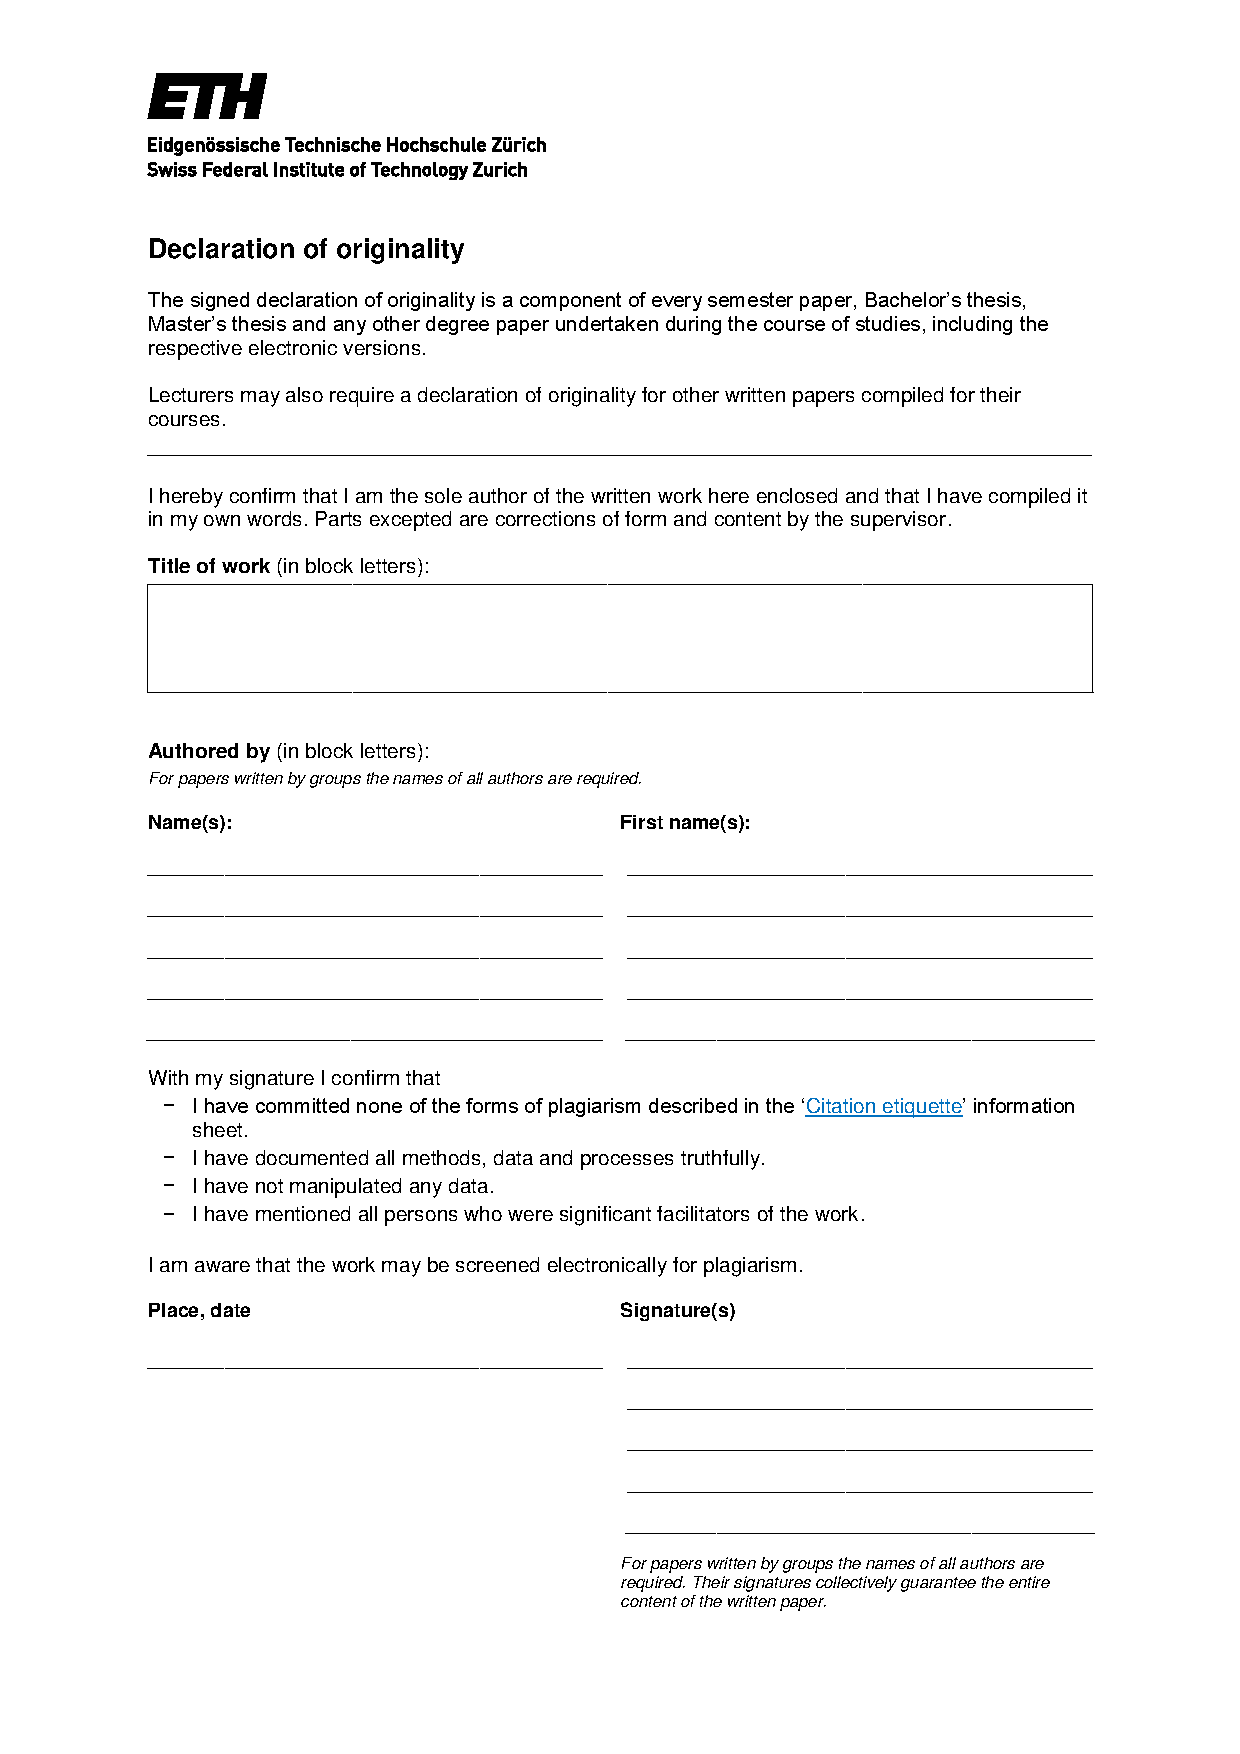
\includegraphics[width=\textwidth]{Figures/declaration-originality.pdf}
\end{figure}

%----------------------------------------------------------------------------------------
%  ABSTRACT PAGE
%----------------------------------------------------------------------------------------

\begin{abstract}
\addchaptertocentry{\abstractname} % Add the abstract to the table of contents
Brief description of the thesis. Capture readers' interest. Mention/summarize everything that was done in the thesis.
\end{abstract}

%----------------------------------------------------------------------------------------
%  ACKNOWLEDGEMENTS
%----------------------------------------------------------------------------------------

\begin{acknowledgements}
\addchaptertocentry{\acknowledgementname} % Add the acknowledgements to the table of contents
\begin{itemize}
\itemsep0em
  \item Supervisors
  \item Professor
  \item Vasilis
  \item Joao
  \item Octave
  \item FullSWOF\_2D
  \item Inkscape
\end{itemize}
\end{acknowledgements}


%----------------------------------------------------------------------------------------
%	ABBREVIATIONS
%----------------------------------------------------------------------------------------

\begin{abbreviations}{ll} % Include a list of abbreviations (a table of two columns)

\textbf{FVM} & \textbf{F}inite \textbf{V}olume \textbf{M}ethod\\


\end{abbreviations}

%----------------------------------------------------------------------------------------
%  TABLE OF CONTENTS
%----------------------------------------------------------------------------------------

\tableofcontents

%----------------------------------------------------------------------------------------
%  THESIS BODY
%----------------------------------------------------------------------------------------

\mainmatter % Begin numeric (1,2,3...) page numbering

\pagestyle{thesis} % Return the page headers back to the "thesis" style

% Include the chapters of the thesis as separate files from the Chapters folder
% Uncomment the lines as you write the chapters

\chapter{Introduction}
\label{chp:introduction}
%----------------------------------------------------------------------------------------

% Define some commands to keep the formatting separated from the content 
\newcommand{\keyword}[1]{\textbf{#1}}
\newcommand{\tabhead}[1]{\textbf{#1}}
\newcommand{\code}[1]{\texttt{#1}}
\newcommand{\file}[1]{\texttt{\bfseries#1}}
\newcommand{\option}[1]{\texttt{\itshape#1}}

%----------------------------------------------------------------------------------------



Flooding and inundation have dramatically increased in the last years due to climate change.
The frequency, as well as the magnitude of extreme rain events, leading to major inundations, have grown, making our capability to predict occurrence and effects more unreliable.
To limit risks and damage, novel control, mitigation and warning measures are needed.
Design and implementation of these need preliminary study of the situation based on data and information.
Unfortunately, these are often not available, or not in the amount required for carrying out preliminary studies.

Nowadays simulation offers a valid and very powerful tool for dealing with this problem.
Hydrological numerical models of catchments can be built, where depending on the degree of detail required different processes are implemented: infiltration, evaporation, erosion, etc.
Depending on the degree of detail chosen more or less accurate models can be achieved.
These models are mainly based on topographical data of the catchment in question, which are then refined by assigning friction coefficients values, infiltration capacity values, hydraulic conductivity values, porosity values to the different zones of the catchment.
Such models need to be calibrated.
This means that by using optimization algorithms the parameters of the model are varied within certain ranges in order to reproduce at best a recorded output (e.g. river outlet hydrograph) generated from "known" initial conditions (e.g. initial soil saturation) and inputs (e.g. the recorded hyetograph).
Once the model is calibrated it can be used to generate new data, from which new information about the given system can be learned and from which other conditions and new situations can be tested.

The main drawback of simulation lays in its very high computational burden.
For calibration alone several runs of the model are required.
Every simulation can last from some minutes up to several hours, depending on the complexity of the model, the type of computer where the simulations are run, the duration of the event simulated, the resolution used for the model, etc.
Once the model is calibrated several more runs are necessary in order to generate the desired dataset.
The number of runs depends on the kind of study one would like to carry out.
For uncertainty analysis for example, up to some thousands of simulations can be run, in order to study the influence that the variation of a parameter of the model (or its uncertain determination) has on the output.\\

\ldots\\



\seb{Rearrange and somehow integrate the two previous sections in order to produce a global introduction. Introduce the following section "Emulation", a brief introduction about emulation}

% ---------------------------------------------------------------------------------------------------
% ===================================================================================================
\section{Definition of goals}
% ===================================================================================================

Focus on emulation subject.

\begin{itemize}
\itemsep0em
  \item explain what is emulation
  \item use both terms \textit{surrogate model} and \textit{emulator}
  \item mention \textit{EmuMore} project
  \item give emulation examples
\end{itemize}


% ==============================================================================
\section{Emulation}
% ==============================================================================

\begin{itemize}
\itemsep0em
  \item define the goals of this thesis
  \item state the questions which should be answered withing this thesis. Try to close the loop in the conclusions chapter (cf. Thesis example Jörg)
  \item what readers should expect from the thesis
  \item mention reproducibility, open softwares
  \item include a scheme with the \emph{emulation workflow}
\end{itemize}









\chapter{Material and Methods}
\label{chp:material_methods}
% ---------------------------------------------------------------------------------------------------

% ===================================================================================================
\section{Regression and interpolation methods}
% ===================================================================================================

\begin{itemize}
\itemsep0em
  \item explain the work done on regression and interpolation
  \item explain their relation with emulation
  \item explian extrapolation, when it can be done and how reliable it can be
\end{itemize}


% ===================================================================================================
\section{Development of \textit{FullSWOF\_2D} interaction tools}
% ===================================================================================================

\begin{itemize}
\itemsep0em
  \item explain the work done
  \item list the functions developed and their function
  \item mention \textit{fswof2d} repository
  \item explain how to install the package?? \noteseb{does this make sense here?? should go in the README}
\end{itemize}

As already mentioned in section \colseb{mention which section} \textit{FullSWOF\_2D-v1.07.00} was chosen as \emph{overland flow simulator} in order to generate the required datasets.
\textit{FullSWOF\_2D} needs at least three input files in order to run simulations:

\begin{itemize}
\itemsep0em
  \item \textit{topography}: a text file specifying the topography of the domain
  \item \textit{parameters}: a text file specifying the values set for the simulation parameters
  \item \textit{huv\_init}: a text file defining the initial conditions of the problem (initial water height and initial water velocity at every point of the grid)
\end{itemize}

In order to generate these files, interaction functions were developed with the open source tool \textit{Octave 4.2.1} \autocite{octave_community_gnu_2018}.
The interaction functions were grouped into the Octave package \textit{fswof2d} available at \url{https://bitbucket.org/binello7/fswof2d}.\\

The package includes the following functions, all of which are distributed under \textit {GPLv3} license \autocite{smith_quick_2014}.

\begin{itemize}
\itemsep0em
  \item center2node.m
  \item csec\_channel2lvlsym.m
  \item dataconvert.m
  \item extrude\_csec.m
  \item huv2file.m
  \item matplotlib\_cm.m
  \item node2center.m
  \item params2file.m
  \item read\_params.m
  \item topo2file.m
\end{itemize}

% ---------------------------------------------------------------------------------------------------
\subsection*{center2node.m}
% ---------------------------------------------------------------------------------------------------
\textit{function x = center2node (cx, x0)}\\



% ---------------------------------------------------------------------------------------------------
\subsection*{node2center.m}\\
% ---------------------------------------------------------------------------------------------------
\textit{function cx = node2center (x)}\\

\textit{FullSWOF\_2D} uses a regular uniform grid in order to solve the \emph{shallow water equation} with the finite volume method (FVM).
The equations are solved at the center of every cell.
After creating the vector defining the grid nodes, one can use the \textit{center2node} function to compute the centers of the grid cells.
This is particularly useful because the $(x,y)$ coordinates saved to the \textit{topography} file have to be the coordinates of the cell centers.
A short usage example would be:

\begin{lstlisting}
  # define the domain length in x-direction
  Lx = 100;
  # define the number of nodes
  Nx = 200;
  # create nodes of the regular grid in x-direction
  xn = linspace (0, Lx, Nx);
  # create vector of cell centers
  xc = node2cdenter (xn);
\end{lstlisting}



% ===================================================================================================
\section{Didactic example: emulator \noteseb{appropriate to use emulator here? other suggestions?} of " the weir equation"}
% ===================================================================================================

\begin{itemize}
\itemsep0em
  \item present it as a didactic example
  \item use it to compare GP (prior knowledge) with e.g. deep neural networks: how many points can we have?
  \item mention grid convergence study (results go in the appendix A)
  \item mention problem with FullSWOF boundary conditions
  \item define well results and methodology
\end{itemize}

% ---------------------------------------------------------------------------------------------------
\subsection{Methodology}
% ---------------------------------------------------------------------------------------------------

Short methodology of how the mechanistic emulator of the weir equation was developed, without subdivision into further subsections.


% ---------------------------------------------------------------------------------------------------
\subsection{Results and discussion}
% ---------------------------------------------------------------------------------------------------

Present and discuss briefly the results of this toy emulator.


% ===================================================================================================
\section{Generating the synthetic topography}
% ===================================================================================================

In order to run the simulations necessary for building the \textit{emulator}, a synthetic topography was produced.
The synthetic topography, in comparison with a real one, has the advantage of having a much smoother surface.
This ensures convergence of the solution at lower grid resolution, reducing therefore the simulation runtime.
The procedure to follow in order to build the \textit{emulator} with a real topography would be exactly the same.\\

The synthetic topography was produced using the software \textit{Octave 4.2.1} \noteseb{how to cite this?} \autocite{octave_community_gnu_2018} and the developed package \textit{fswof2d} \noteseb{cite it? how?} in order to export it to a format compatible with \textit{FullSWOF\_2D-v.1.07.00} \autocite{delestre_fullswof:_2014} \noteseb{put the citation every time that it is mentioned?}.
The generated topography is visible in Fig.~\ref{fig:topography}.
It represents a catchment of $\SI{2}{\kilo\meter} \times \SI{2}{\kilo\meter}$ composed of a sloping plane with three Gaussian bumps on the top.
The Gaussian bumps have different heights and widths and generate a \emph{Y-shaped channel} which extends from the upper and left boundary down to the lower boundary.
A paraboloid was added to the plane to promote the accumulation of water in the channel.\\


\begin{figure}[htpb]
  \centering
  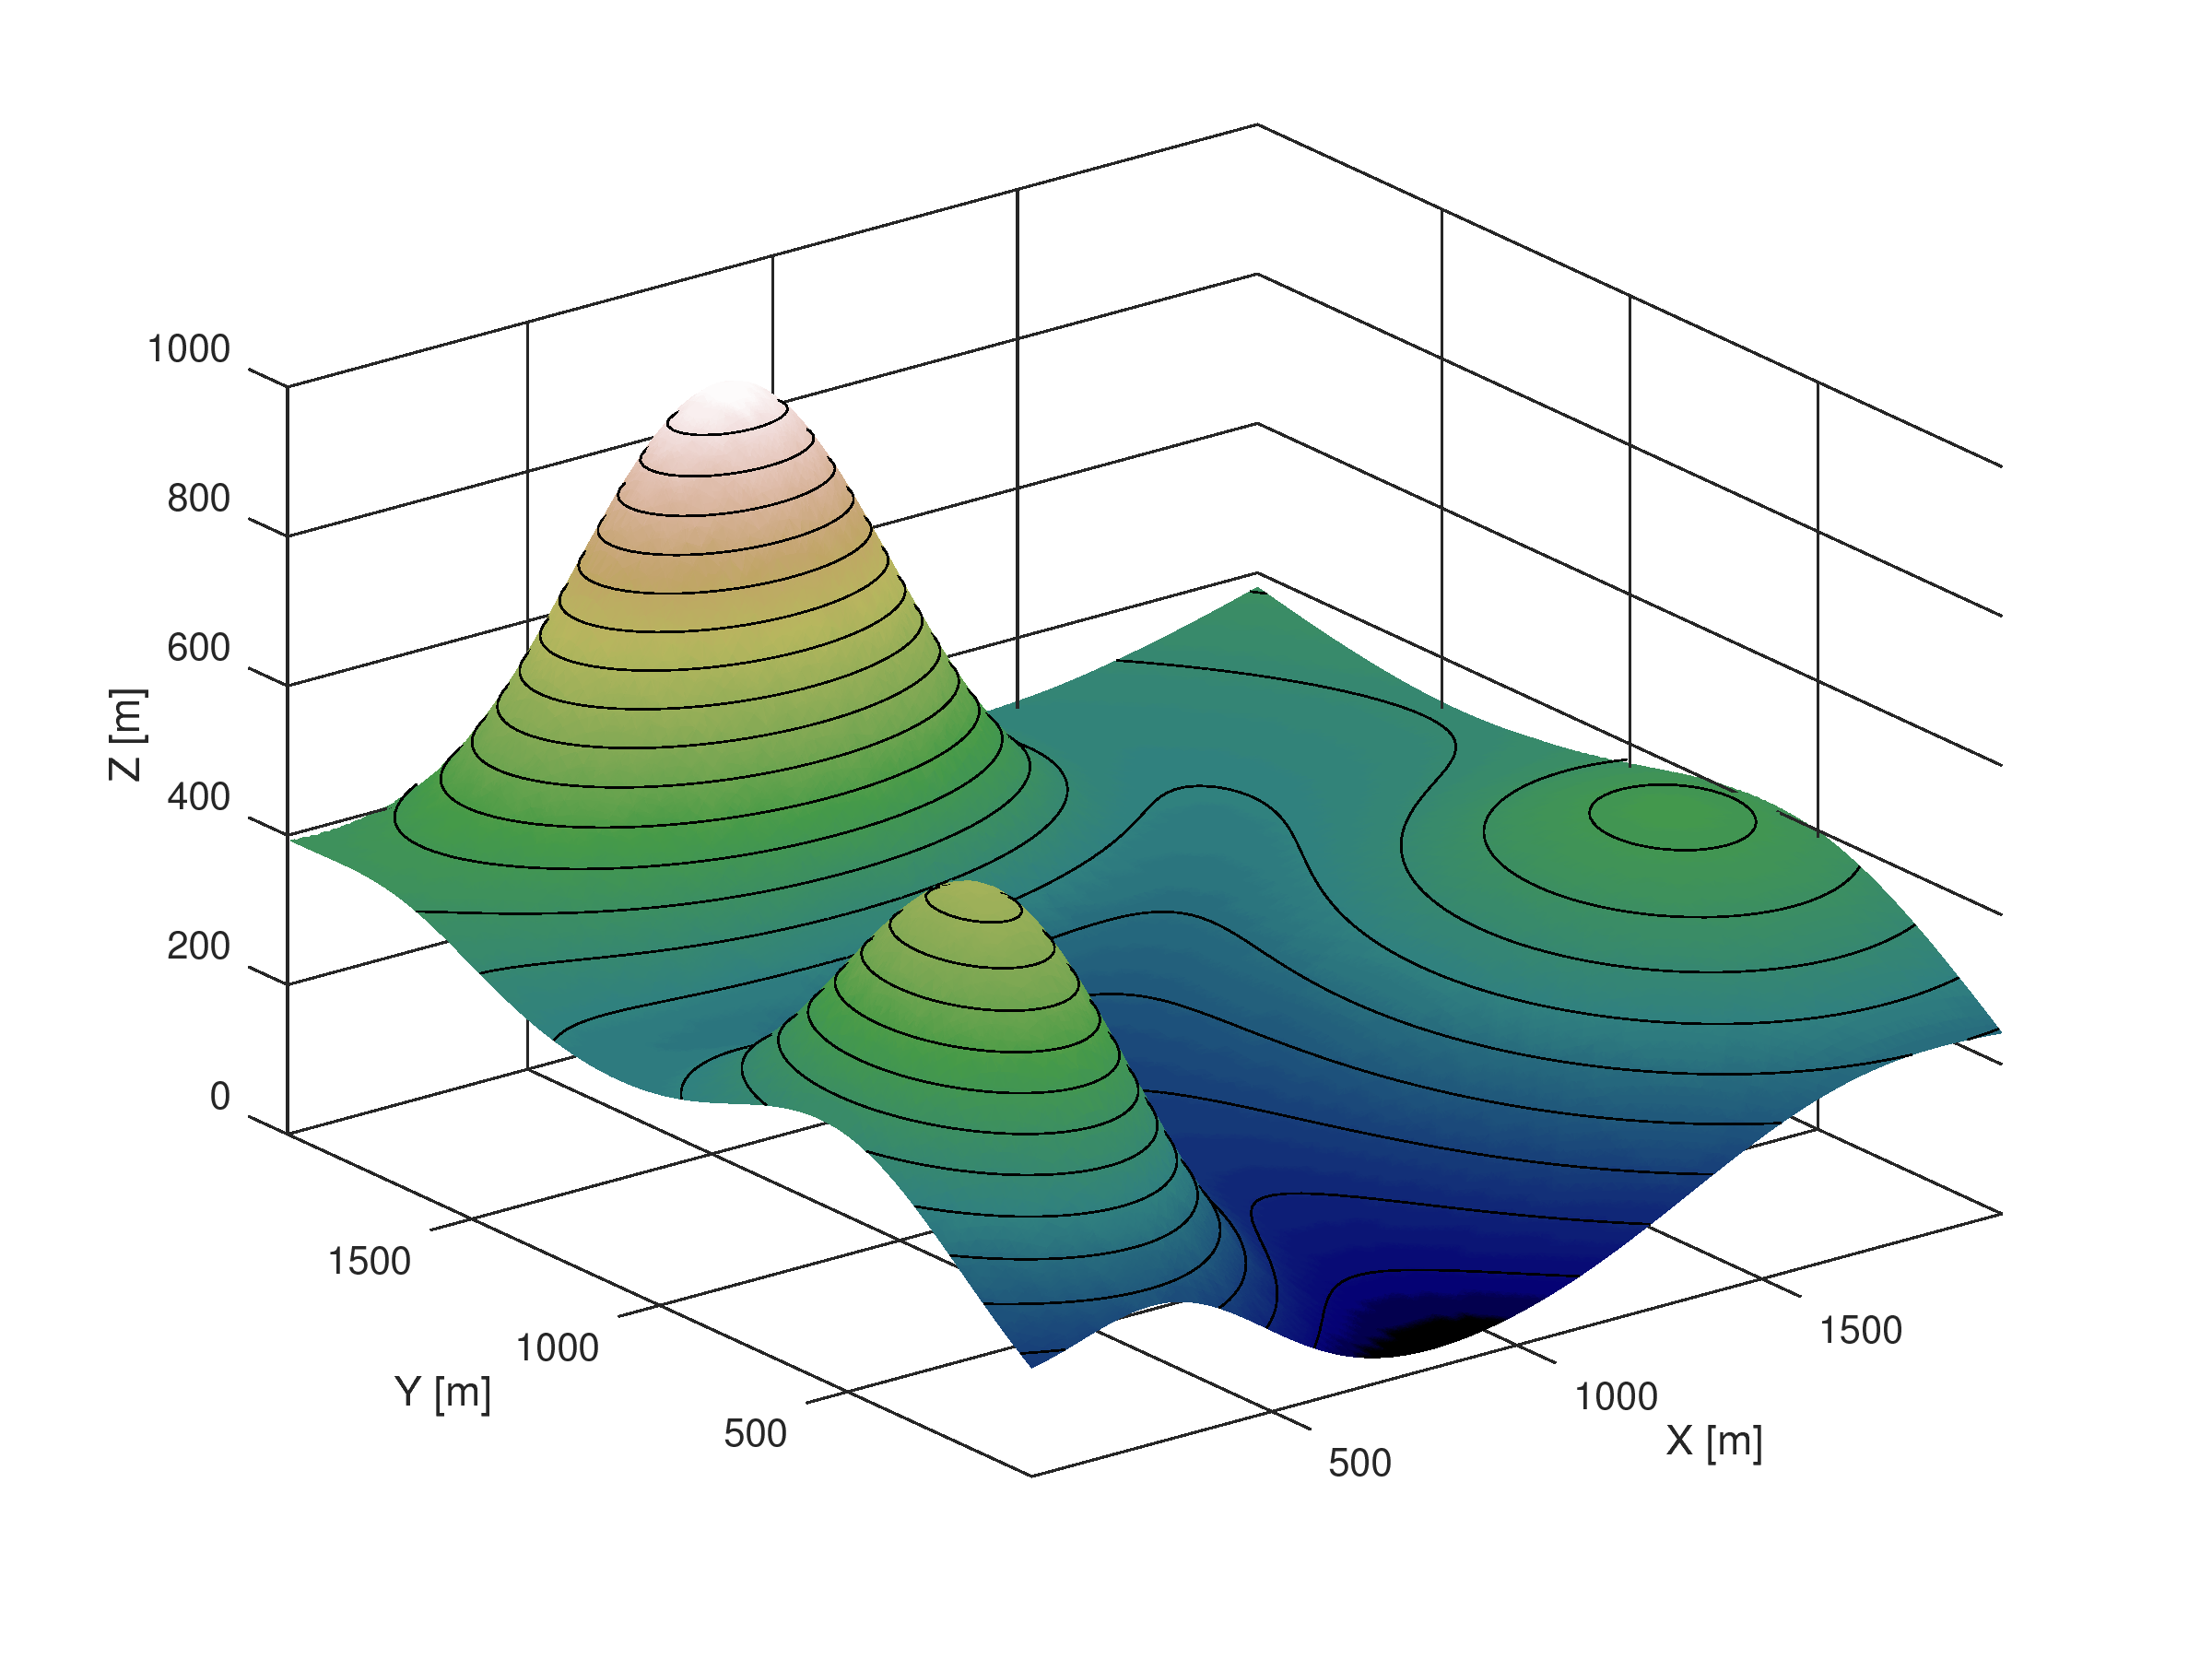
\includegraphics[width=0.7\textwidth]{Figures/topography.png}
  \caption{Synthetic topography composed of three Gaussian bumps on a sloping plane.}
  \label{fig:topography}
\end{figure}

\begin{table}[htpb]
  \centering
  \caption{Parameters and setting fixed for all simulations.}
  \label{tab:simulations_parameters}
  \begin{threeparttable}
    \begin{tabular}{lrl}
      \toprule
      \textbf{Parameter} & \textbf{Value} & \textbf{Units} \\
      \midrule
      Domain x-length                          &    $2'000$           & \si{\meter}   \\
      Domain y-length                          &    $2'000$           & \si{\meter}   \\
      Number of cells x                        &    $100$             & --   \\
      Number of cells y                        &    $100$             & --   \\
      Friction coefficient\tnote{*}            &    $0.03$            & \si{s.m^{-1/3}}\\
      Crust thickness\tnote{*}                 &    $1$               & \si{\meter}\\
      Crust hydraulic conductivity\tnote{*}    &    $2\cdot 10^{-6}$  & \si{\meter\per\second}\\
      Soil hydraulic conductivity\tnote{*}     &    $2\cdot 10^{-6}$  & \si{\meter\per\second}\\
      Soil suction head\tnote{*}               &    $0.09$      & \si{\meter}\\
      Soil maximum infiltration rate\tnote{*}  &    $19.8$      & \si{\milli\meter\per\hour}\\
      \bottomrule
    \end{tabular}
    \begin{tablenotes}
      \item[*] Parameters spatially distributed.
    \end{tablenotes}
  \end{threeparttable}
\end{table}


% ===================================================================================================
\section{Generating the datasets}
% ===================================================================================================

The dataset required for building the emulator was generated by running \num{50} simulations with different combinations of the variables \emph{rain intensity} ($I$) and \emph{initial soil saturation} ($\theta_i$).
The initial soil saturation, being a spatially distributed variable, was kept uniform over the whole domain.
The rain intensity was also uniformly applied over the domain, also since \textit{FullSWOF\_2D}, at this stage of development, only allows for uniformly distributed rain events.
\num{5} different initial saturations in the $[\numrange{0}{1}]$ interval and \num{10} rain intensities in the \SIrange{10}{35}{\milli\metre\per\hour} interval were taken and all their possible combinations were used as inputs for the simulations.
This data constitute the \emph{training dataset} for the emulator.
A \emph{test dataset} and a \emph{validation dataset} were also generated.
These datasets can be found in the Appendix~\ref{AppendixB}.

Some parameters, namely those specific for the catchment in questions, were kept constant over all of the simulations.
This are summarized in Tab.~\ref{tab:simulations_parameters}.
The parameters marked with * are those \emph{spatially distributed}, meaning that a different value could be set for every cell.
For simplicity, a spatially uniform catchment was used, therefore the values from the table are valid for the whole domain.


\begin{figure}[htpb]
  \centering
  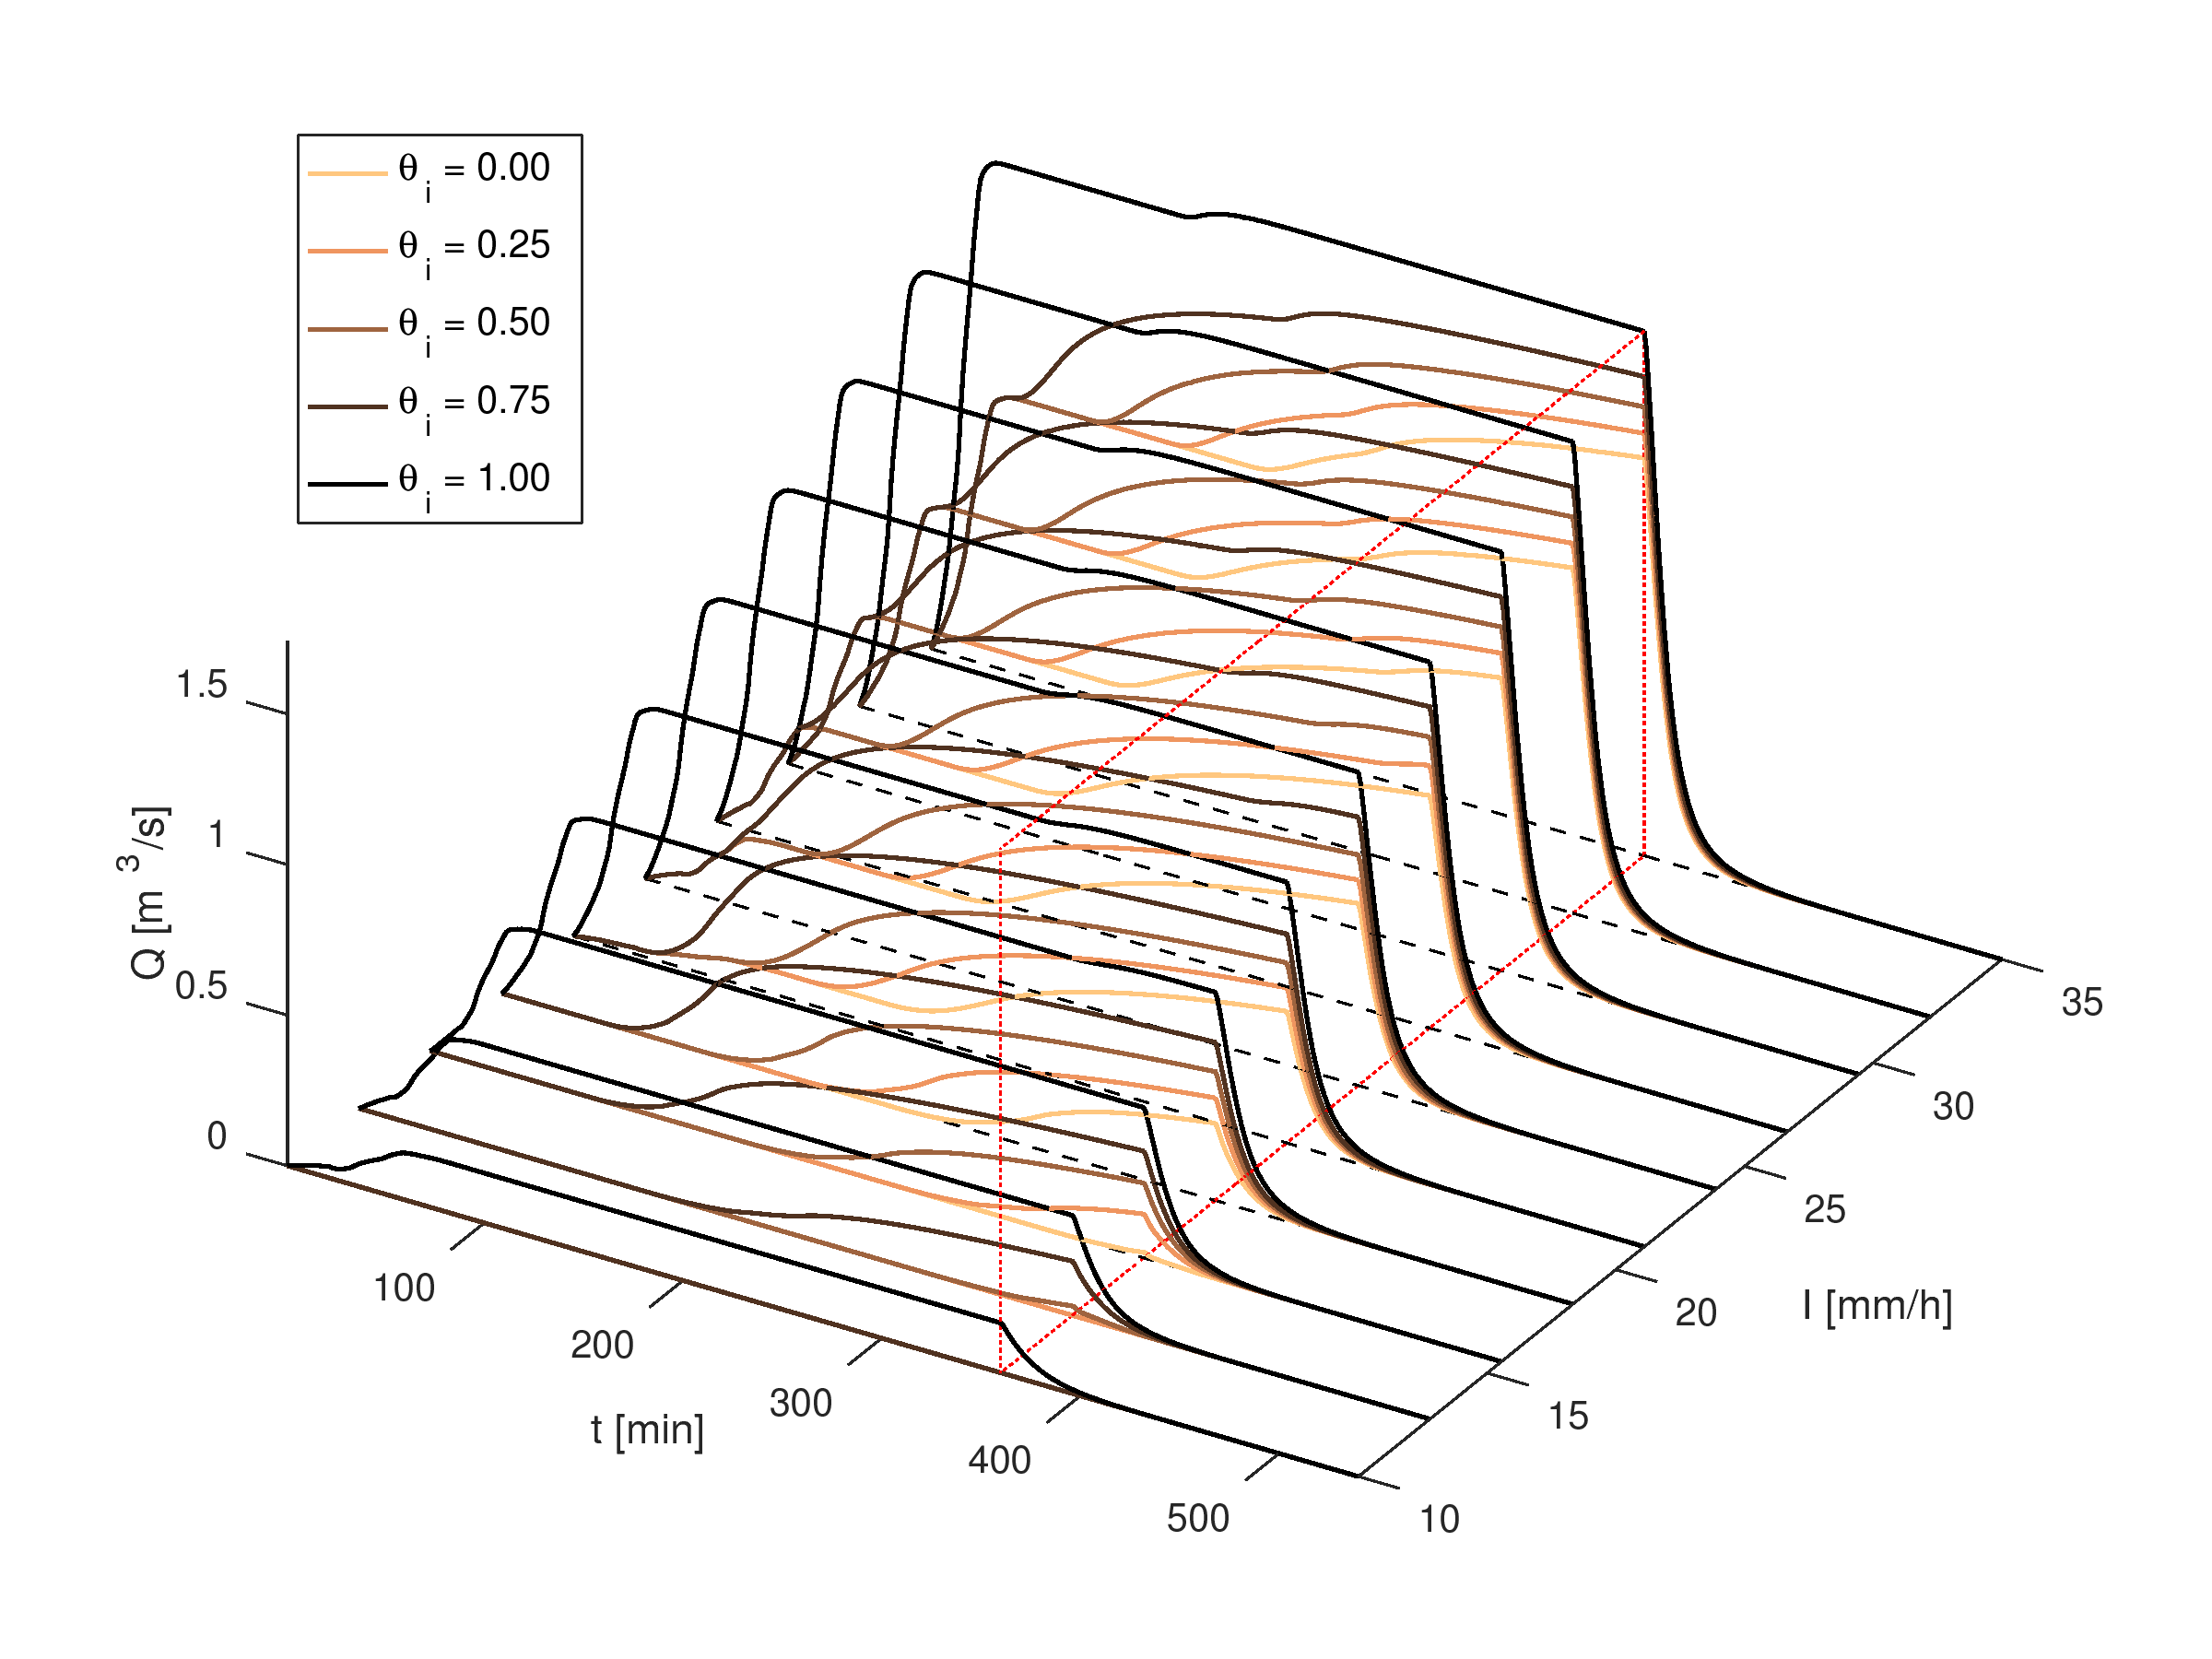
\includegraphics[width=0.75\textwidth]{Figures/hydrographs3d.png}
  \caption{Response hydrographs of the \num{50} simulations at the catchment outlet.}
  \label{fig:hydrographs3d}
\end{figure}


% ===================================================================================================
\section{Building the emulator}
% ===================================================================================================

% ---------------------------------------------------------------------------------------------------
\subsection{Classification emulator}
% ---------------------------------------------------------------------------------------------------

% ---------------------------------------------------------------------------------------------------
\subsection{Time-to-threshold emulator}
% ---------------------------------------------------------------------------------------------------



\chapter{Results}
\label{chp:results}
% ---------------------------------------------------------------------------------------------------


\begin{itemize}
\itemsep0em
  \item emulator should never underestimate danger (what type of error is this? we want to avoid it absolutely)
  \item try to perform GP interpolation. If it does not work, explain why polynomial interpolation (no time)
  \item use emulator with uncertainty in the $I$ and $\theta_i$. Perform uncertainty quantification
\end{itemize}

% ===================================================================================================
\section{Classification emulator}
% ===================================================================================================

Results for the classification emulator
\begin{itemize}
  \item show classification with 3 different $Q_!$
  \item perform testing 
\end{itemize}

\begin{figure}[htpb]
  \centering
  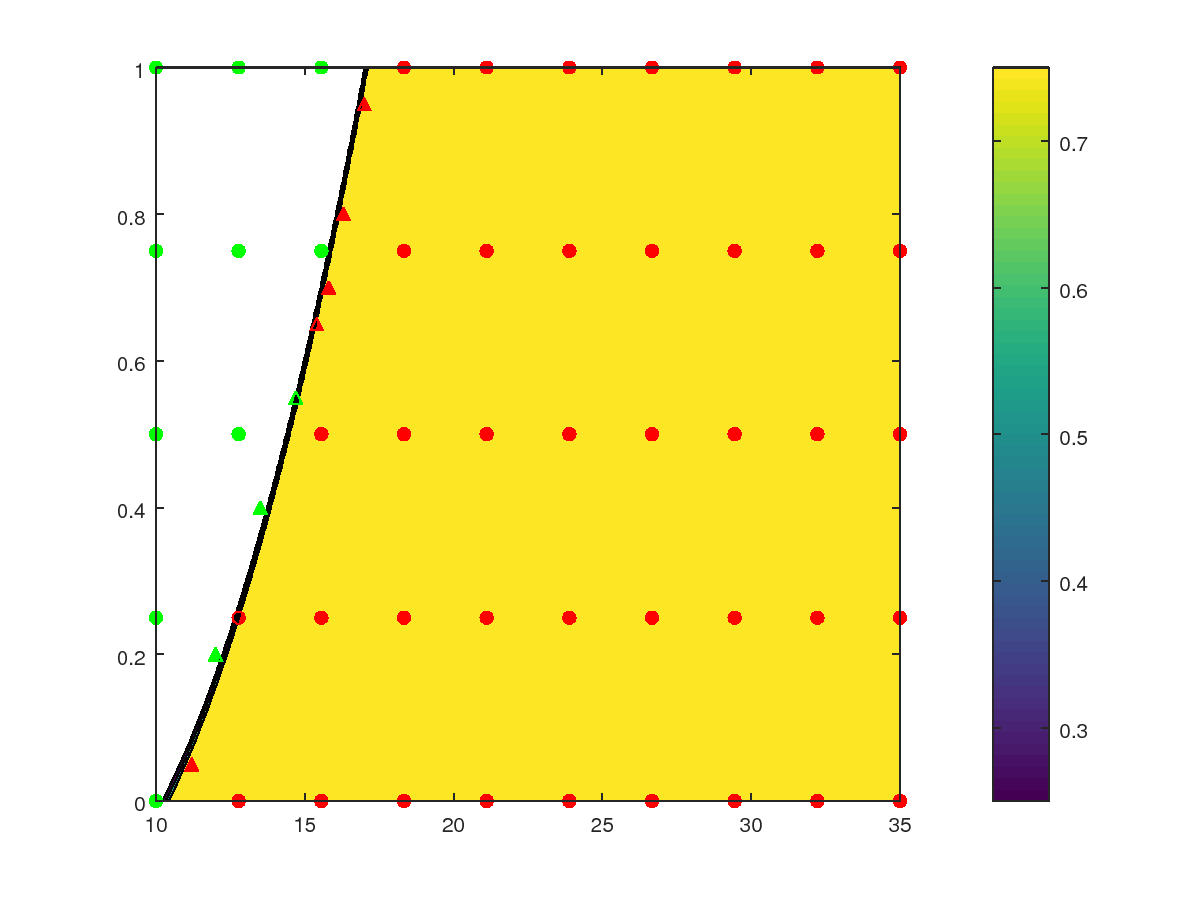
\includegraphics[width=0.75\textwidth]{Figures/classification.png}
  \caption{Binary classification emulator: events reaching $Q_!$ (red) and events not reaching $Q_!$ (green) for $Q_! = XX.X$.}
  \label{fig:classification_Q1}
\end{figure}

% ---------------------------------------------------------------------------------------------------
\subsection{Classification performance}
% ---------------------------------------------------------------------------------------------------


% ===================================================================================================
\section{Time-to-threshold emulator}
% ===================================================================================================

\begin{figure}[htpb]
  \centering
  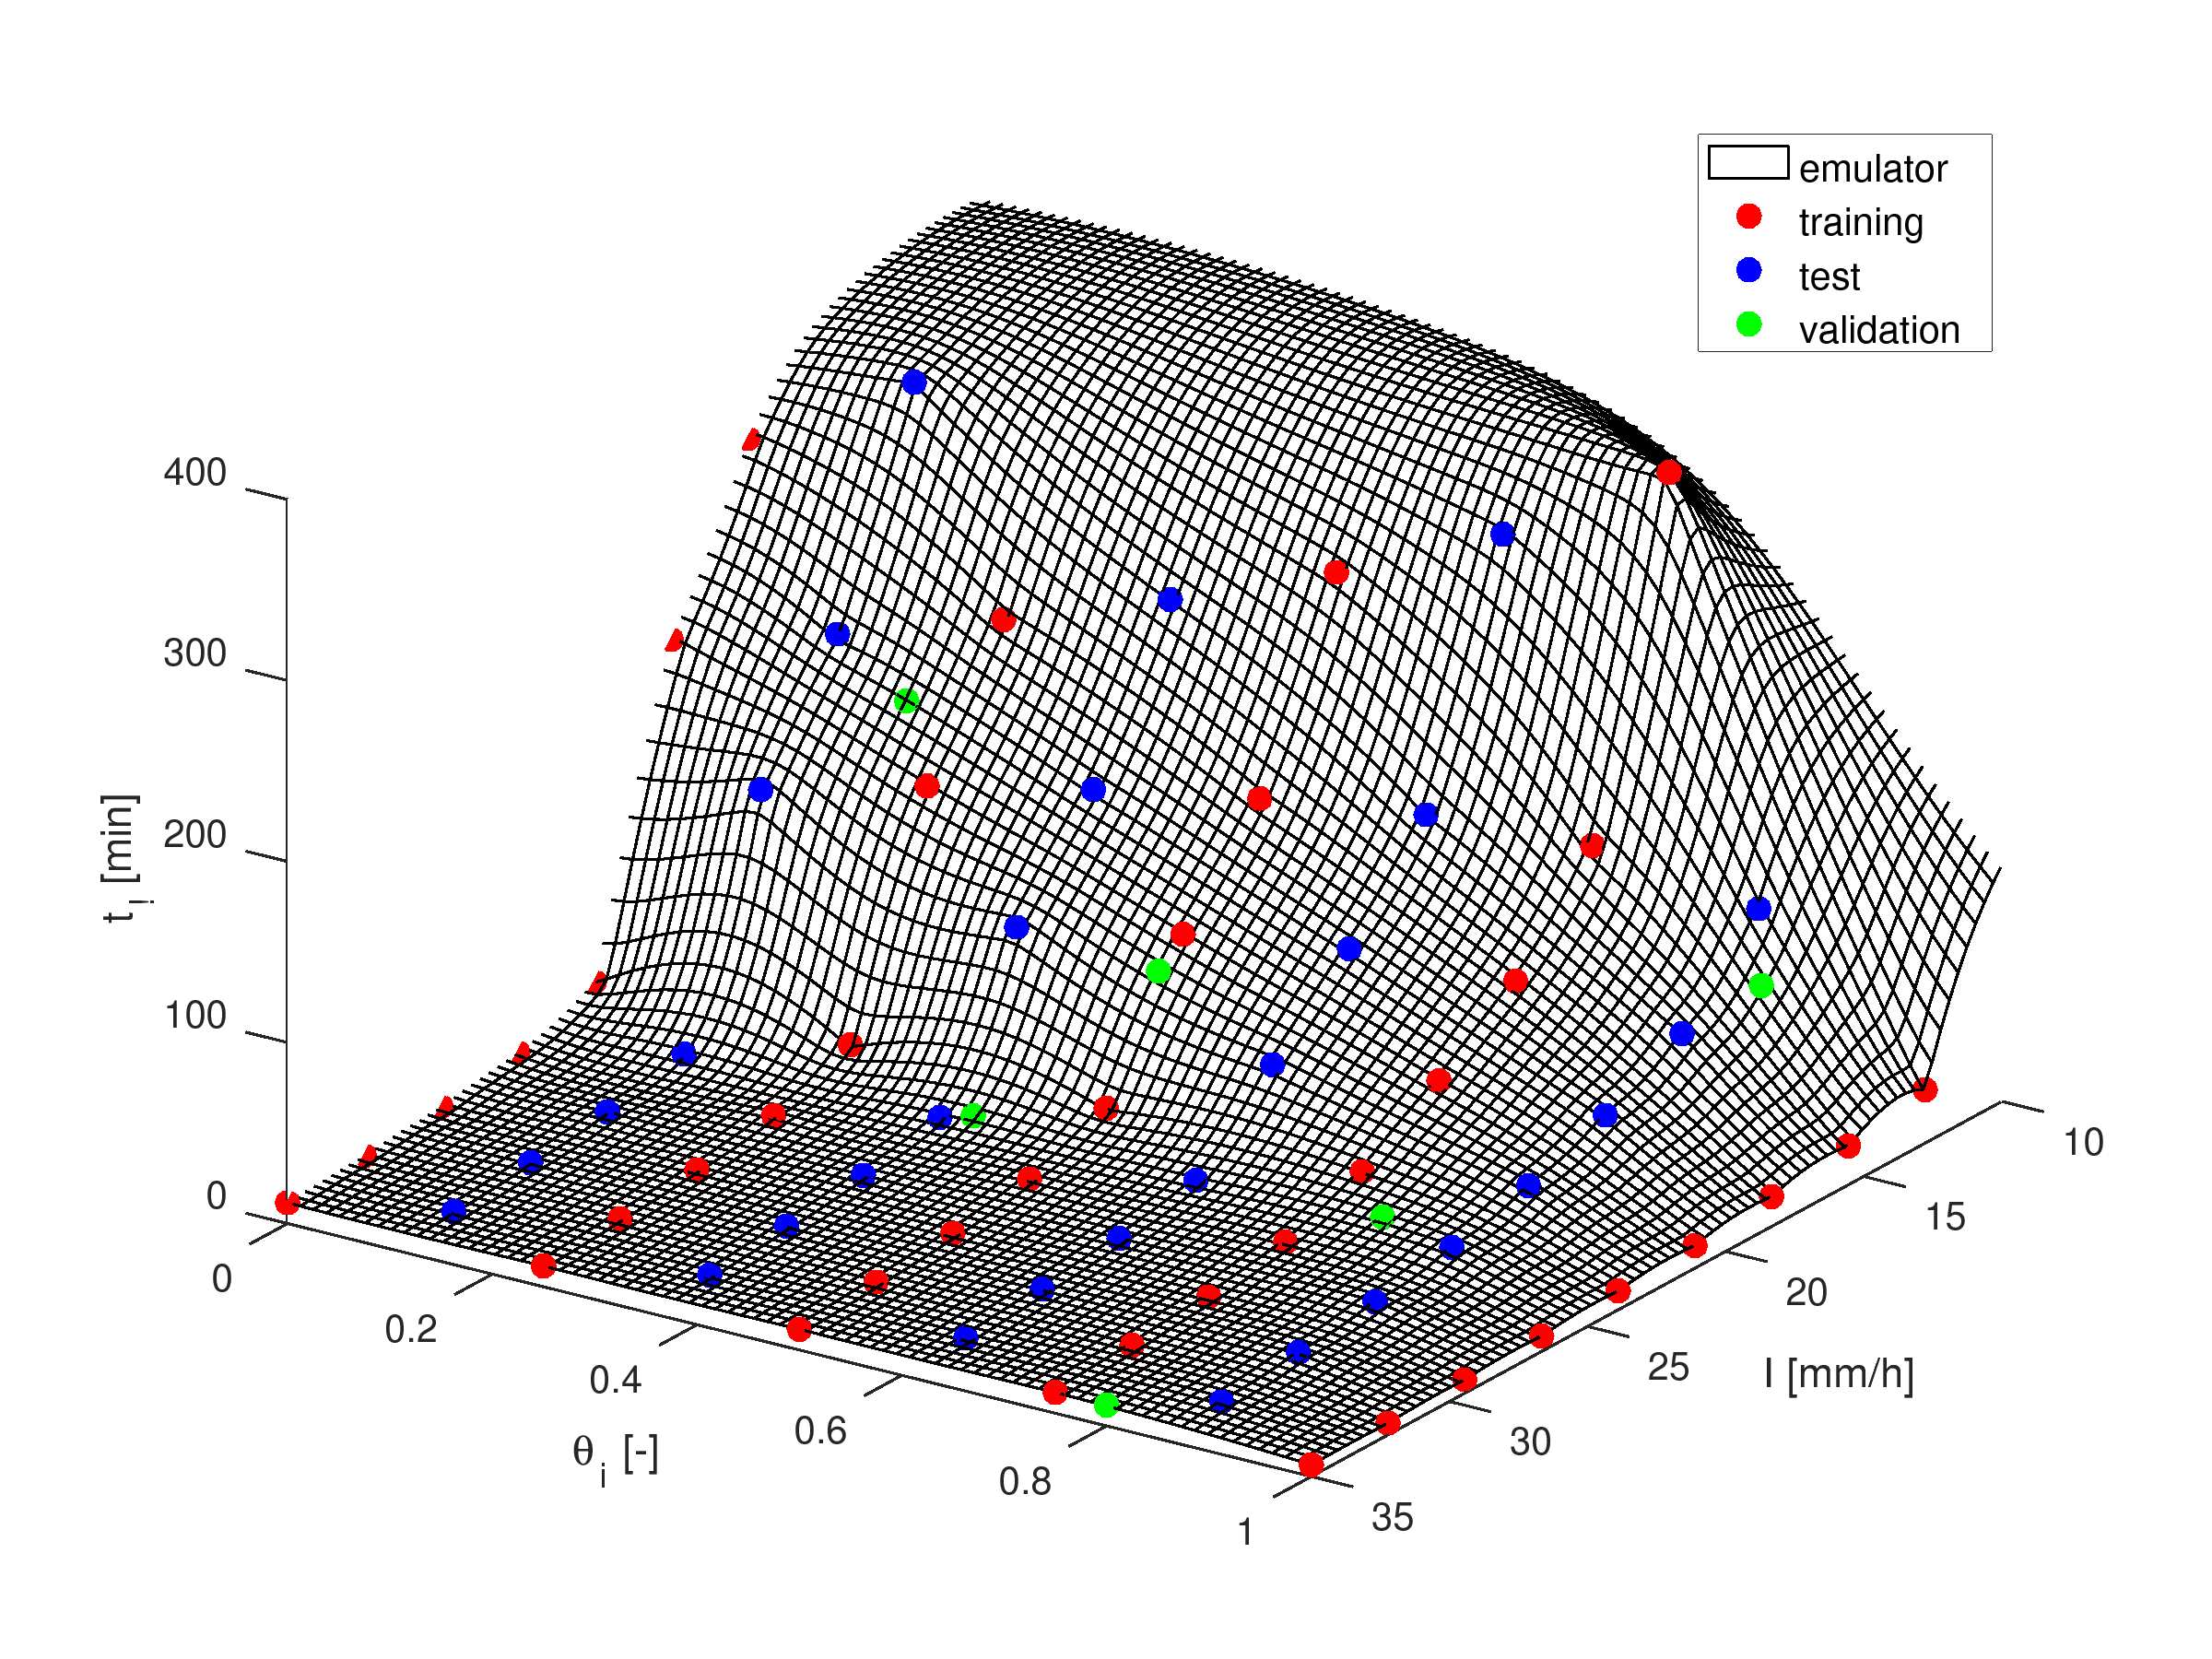
\includegraphics[width=0.7\textwidth]{Figures/emulator.png}
  \caption{Time-to-threshold emulator: training (red), test (blue) and validation (green) datasets and the emulator producing the intrapolation response.}
  \label{fig:}
\end{figure}

% ---------------------------------------------------------------------------------------------------
\subsection{Time-to-threshold prediction performance}
% ---------------------------------------------------------------------------------------------------

\begin{table}[htpb]
  \centering
  \caption{Emulator performance on \emph{test} and \emph{validation} data}
  \label{table label}
  \begin{tabular}{lcc}
    \toprule
     & \textbf{MAE [\si{\minute}, \si{\percent}]} & \textbf{RMSE [\si{\minute}, \si{\percent}]} \\
    \midrule
    \textbf{test} & val & val \\
    \textbf{validation} & val & val \\
    \bottomrule
  \end{tabular}
\end{table}


% ---------------------------------------------------------------------------------------------------
\subsection{Parameters uncertainty propagation}
% ---------------------------------------------------------------------------------------------------






\chapter{Discussion}
\label{chp:conclusions}



\chapter{Conclusions}
\label{chp:outlook}




%individual results are probably being discussed in 3.1.2 and 3.2.2

%Here, you could provide a joint discussion, maybe discussion common features/insight for both case studies. FullSwof, GPs as tools vs. "simple" emulators such as response surfaces/lin. methods.

%Also, you could move the next steps/outlook part here.



%probably move bullet points 2 and 3 to discussion section and have Conclusion as summarizing section, re-stating the problem, the general approach, the main results (Answers to Research questions). and brief summary of future work.


%5.1. Answers to research questions

%5.2. Open questions


%s of this thesis.

%You can stay with "Goals", or break it down into different "objectives"/sub-goals, if needed.

%From goals/objectives, usually research questions are derived. These should be as specific as possible, so you can write a concise answer.





%The work done on emulation 

This thesis follows a storyline, which connects up the dots, resulting in a prelude to emulation for near-time flood prediction.
Venturing in a completely new field, that of emulation, opened me up a whole new world.
This itinerary through emulation, after clearing up some initial doubts, made me realize its true potential.
Emulation can have great applicability, especially in the engineering fields.
Engineering often has to tackle repetitive problems, which solution can be found only iteratively.
Emulation can provide alternative new ways to solve such problems.
Once an appropriate emulator for a specific task is built, this can provide fast answer to the problem of interest.
Emulation can be performed at almost no cost: it requires neither special tools nor special investments.
The work done on this thesis demonstrate it.\\

In spite of its simplicity, the first case study was for me a very didactic one.
The weir equation, commonly used in hydraulic engineering, proved to be a fair approximation of the relation discharge-height over the weir, although flexible non parametric interpolation techniques have shown to produce more accurate estimates when an adequate number of observations is available.
This case study also shows the potential of numerical simulation in replacing the realization of laboratory experiments, with the potential of reducing future research costs and time.\\

Although the methodology in the second case study appears more complex than the one adopted in the first one, the high level of abstraction and generalization of the presented workflow allows to apply the proposed early flood warning system to real situations with only slight modifications. These especially concerns the assessment of the emulator performance. Still, the partial accuracy assessment conducted reported excellent performance, especially with regards to the estimation of the time period before a flood occurs. \\

In conclusion, this thesis shows the benefit of conjugating the accuracy of numerical simulation with the huge enhancement in computing time provided by emulators. In the engineering field, promising research areas may include uncertainty propagation, sensitivity analysis and models optimization or calibration, which are actually hampered by the excessive computational burden of numerical simulation. 


 
% - automatization
% - to bridge a gap
% innovation

 
 

 




















%----------------------------------------------------------------------------------------
%  BIBLIOGRAPHY
%----------------------------------------------------------------------------------------

\printbibliography[heading=bibintoc]

%----------------------------------------------------------------------------------------
%  APPENDIX
%----------------------------------------------------------------------------------------

\appendix % Cue to tell LaTeX that the following "chapters" are Appendices

% Include the appendices of the thesis as separate files from the Appendices folder
% Uncomment the lines as you write the Appendices

% Appendix A

\chapter{Frequently Asked Questions} % Main appendix title

\label{AppendixA} % For referencing this appendix elsewhere, use \ref{AppendixA}

\section{How do I change the colors of links?}

The color of links can be changed to your liking using:

{\small\verb!\hypersetup{urlcolor=red}!}, or

{\small\verb!\hypersetup{citecolor=green}!}, or

{\small\verb!\hypersetup{allcolor=blue}!}.

\noindent If you want to completely hide the links, you can use:

{\small\verb!\hypersetup{allcolors=.}!}, or even better: 

{\small\verb!\hypersetup{hidelinks}!}.

\noindent If you want to have obvious links in the PDF but not the printed text, use:

{\small\verb!\hypersetup{colorlinks=false}!}.

% Appendix B

\chapter{Early flood warning}
\label{AppendixB}

\section{Training dataset}
\label{sec:training_dataset}

\begin{table}[htpb]
  \centering
  \caption{Emulator training dataset}
  \label{tab:training_dataset}
  \begin{tabular}{lccc}
    \toprule
     & \textbf{1} & \textbf{2} & \textbf{3}\\
    \midrule
    $\bm{I}$ \textbf{[\si{\milli\meter\per\hour}]} & val & val & val \\
    $\bm{\theta_i}$ \textbf{[--]} & val & val & val \\
    \bottomrule
  \end{tabular}
\end{table}

\section{Testing dataset}
\label{sec:testing_dataset}

\begin{table}[htpb]
  \centering
  \caption{Emulator test dataset}
  \label{tab:test_dataset}
  \begin{tabular}{lccc}
    \toprule
     & \textbf{1} & \textbf{2} & \textbf{3}\\
    \midrule
    $\bm{I}$ \textbf{[\si{\milli\meter\per\hour}]} & val & val & val \\
    $\bm{\theta_i}$ \textbf{[--]} & val & val & val \\
    \bottomrule
  \end{tabular}
\end{table}

\section{Validation dataset}
\label{sec:validation_dataset}

\begin{table}[htpb]
  \centering
  \caption{Emulator validation dataset}
  \label{tab:validation_dataset}
  \begin{tabular}{lccc}
    \toprule
     & \textbf{1} & \textbf{2} & \textbf{3}\\
    \midrule
    $\bm{I}$ \textbf{[\si{\milli\meter\per\hour}]} & val & val & val \\
    $\bm{\theta_i}$ \textbf{[--]} & val & val & val \\
    \bottomrule
  \end{tabular}
\end{table}


\section{Detailed validation performance}

\begin{table}[htpb]
  \centering
  \caption{Emulator performance on every validation point}
  \label{tab:}
  \begin{tabular}{lccc}
    \toprule
     & \textbf{1} & \textbf{2} & \textbf{3}\\
    \midrule
    \textbf{simulated} $\bm{t_!}$ & val & val & val \\
    \textbf{emulated} $\bm{t_!}$ & val & val & val \\
    \bottomrule
  \end{tabular}
\end{table}





%----------------------------------------------------------------------------------------

\end{document}  
